\chapter{Battery Modeling and Emulation}\label{ch:Battery_Modeling_Emulation}
The \textit{Battery} is a complex composition of lethal chemicals that are very hard to handle in terms of safety and maintenance. So, is those petroleum vehicles safe? No, Not at all petroleum products and vehicles are much more dangerous not only in terms of environmental pollution it in terms of safety and measures. Then we should raise the question of what stopping modern engineers to transition from petroleum engines to Battery vehicles. And which wall stopping us from battery usage? Well, to answer all the above questions we need to look back at the evolution of vehicles, the petroleum vehicle fetus came to this world nearly a century ago. Engineers thoroughly studied and learned how to handle petroleum products and petroleum vehicles. Undoubtedly, EVs are the gift of modern technology, but it is essential to study institutionally the battery characteristics and the testing.

It is the prime responsibility of every Electrical engineer who works in EVs/Battery systems to ensure the safety of mankind. Considering all the facts, I have decided to make safety and sophisticated system for engineers to test the BMS and play with BMS without interacting with the physical batteries. The \textit{Part I} of Chapter \ref{ch:Battery_Modeling_Emulation} gives more elaboration about the battery modeling and battery constructional theory. \textit{Part II} facilitates understanding of Battery model implementation and BMS simulation through coding.

\section{Battery Modeling}\label{sec:Batt_Modeling}
This section explains the principles of a technique for calculating the state of charge (SOC) of lithium-ion batteries using two different equivalent circuit designs. It discusses how to use typical measurements to determine these circuits' parameters. The comparison of measurement and computation results reveals good agreement. The first step ignores the effects of temperature and battery age on these parameters \cite{UKEMPT_AHMAD2012}.
\\
The Ampere-counting (Columb counting) method can be used to identify the state of charge (SOC) of a battery if a defined full charge occurs regularly. This technique is based on the amount of charge that is put into or taken out of the battery. The error in the SOC estimation can grow too big and a better solution needs to be discovered in cases where a defined full charge of the battery cannot occur frequently.
A lithium-ion battery's open circuit voltage (OCV) determines the SOC; however, as shown in the figures, this method has an issue with the battery's dynamics.
The electrochemical reactions that occur in a cell prevent the OCV from being measured at the battery terminals. It is necessary to theoretically model the dynamics so that the OCV or SOC may be determined by measuring simply the battery voltage and current at the terminals of the battery. It is necessary to utilize an analogous circuit design for the battery cell for this purpose, and characteristic measurements must be employed to identify the parameters.
\\
This section presents three models: the internal resistance model (IR)\ref{fig:Battery_Equivalent_circuit}(a), the one-time constant model (OTC) \ref{fig:Battery_Equivalent_circuit}(b), and the two-time constants model (TTC) \ref{fig:Battery_Equivalent_circuit}(c). The presented models, which serve as the basis for the model-based SOC calculation, are also evaluated for validity by making comparisons between the model-based simulation data and the measured data\cite{UniPadua_Giacomo}.

\begin{figure}[h]
	\centering
	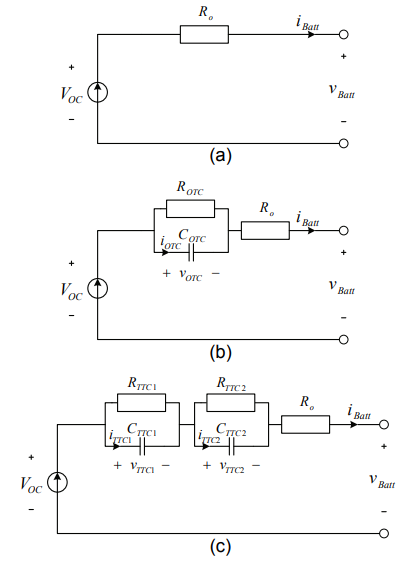
\includegraphics[width=0.5\textwidth]{Chap06/Figures/Batt_Ckt.PNG}
	\caption{Battery equivalent circuit diagrams. (a) internal resistance 
    model (IR), (b) one-time constant model (OTC), (c) two time 
    constants model (TTC) \cite{UKEMPT_AHMAD2012},\cite{UKEMPT_AHMAD2012} }
	\label{fig:Battery_Equivalent_circuit}
\end{figure}

\subsection{Nomenclature of Battery Model}
\begin{enumerate}
	\item \textbf{\textit{\underline{Open Circuit Voltage(OCV) }:}} OCV is measured at the battery's open circuit terminal voltage at various SOC points when the battery is in equilibrium. A polynomial equation is used to determine the nonlinear relationship between SOC and OCV. The figure \ref{fig:Battery_OCV_Vs_Soc} displays an OCV subsystem. Because SOC directly affects OCV's value, the OCV subsystem includes a SOC computation component. The value of OCV controls the regulated voltage source. The voltage curve of the pulse discharge test (PDT) during relaxation can be used to determine the OCV value\cite{Batt_Modeling_Kharisma}.
	\item \textbf{\textit{\underline{Internal Resistanse (R0) }:}} Internal resistance results in a voltage drop in the equivalent circuit. Fig. \ref{fig:Battery_Equivalent_circuit}(a), displays the value of the subsystem R0
	as a function of the input current and SOC. A switchable resistor
	utilized to transmit a resistor's internal value's physical signal.
	From this, one can calculate the amount of internal resistance.
	Instantaneous voltage following the release of the current pulse. 
	The optimal 2-D lookup table is selected using
	the interpolation-extrapolation lookup method for R0's value\cite{Batt_Modeling_Kharisma}.
	\item \textbf{\textit{\underline{Transient Response (R1,C1,R2,C2) }:}} Transient response in this model is represented by RC.
	The transient model is again classified based on the time constant for instance $R1\times C1 = \tau 1$ is a one-time constant model and $R2\times C2 = \tau 2$  is the two-time constant model; Figure \ref{fig:Battery_Equivalent_circuit}(b) and Figure \ref{fig:Battery_Equivalent_circuit}(c). Increasing the Time constant model will serve as a realistic model battery\cite{Batt_Modeling_Kharisma}.
\end{enumerate}

\begin{figure}[h]
	\centering
	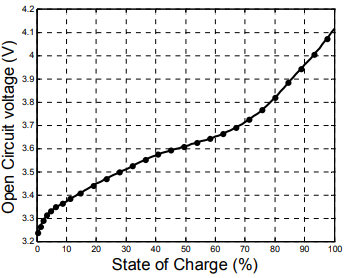
\includegraphics[width=0.5\textwidth]{Chap06/Figures/Batt_OCV_SOC.PNG}
	\caption{Battery OCV Vs Soc for SLPB120216216 Cell \cite{UKEMPT_AHMAD2012}}
	\label{fig:Battery_OCV_Vs_Soc}
\end{figure}

\subsection{IR Model :}
the IR model as shown in Figure r\ref{fig:Battery_Equivalent_circuit} (a), and 
described by Equation \ref{eq:Batt_IR_equation} implements an ideal voltage 
source VOC that represents the open-circuit voltage (OCV) 
of the battery, and an ohmic resistance to describe 
the internal resistance \cite{UKEMPT_AHMAD2012}. Both resistance and open-circuit 
voltage VOC are functions of SOC, state of health (SOH) 
and temperature. $I_{Batt}$ is the battery output current with a 
positive value when discharging, and a negative value when 
charging, $V_{Batt}$ is the battery terminal voltage\cite{UKEMPT_AHMAD2012}.

\begin{equation}\label{eq:Batt_IR_equation}
    V_{Batt} = V{OC} - R_{0}\times I_{Batt}
\end{equation}
Given that the transient is not represented by the IR model
Lithium-ion cell behavior is not suited for the
precise SOC calculation for any dynamical operation
(variable load).

\subsection{One-Time Constant Model }
A parallel RC is added by the OTC model.
Network connected in series to the IR's internal resistance R0
model to approximate the lithium-ion battery's dynamic behavior.
As shown in Figure \ref{fig:Battery_Equivalent_circuit} (b), it mainly 
consists of three parts including the voltage source $V_{OC}$, the 
ohmic resistance R0, and $R_{OTC}$,$C_{OTC}$ to describe the battery 
transient response during charging or discharging. $\textit{V}_{OTC}$ is 
the voltage across $C_{OTC}$; $i_{OTC}$ is the current that flows in 
$C_{OTC}$ \cite{UKEMPT_AHMAD2012} $\dot{\textit{V}_{OTC}}$ is the iterative voltage of OTC model. The electric behavior of the OTC model can be 
expressed by Equations \ref{eq:OTC_Voltage } and \ref{eq:OTC_Batt_Voltage } \cite{UKEMPT_AHMAD2012} in continuous time \cite{UniPadua_Giacomo}: 

\begin{equation}\label{eq:OTC_Voltage }
    \dot{ V_{OTC}} = \frac{-1}{R_{OTC}\times C_{OTC}} V_{OTC} + \frac{1}{C_{OTC}} i_{Batt}
\end{equation}
\begin{equation}\label{eq:OTC_Batt_Voltage }
    V_{Batt} = V_{OC} -  \frac{1}{C_{OTC}} V_{OTC} - R_{0}\times i_{Batt}
\end{equation}
The equation\ref{eq:Discrete_OTC_Voltage } and \ref{eq:Discrete_OTC_Batt_Voltage } (where: $T_S$ sampling period, $T_s$ and $\tau_{OTC}$  time constant. ) represents the discrete time voltages of the one-time constant model, They are very much helpful for the advanced algorithms to calculate the SoC such as Kalman, Extended Kalman etc.
\begin{equation}\label{eq:Discrete_OTC_Voltage }
    V_{OTC,k+1} = e^{\frac{-T_{s}}{\tau_{otc}}} V_{OTC,k} + R_{OTC}\left(1- e^{\frac{-T_{s}}{\tau_{otc}}}\right) i_{Batt,k}
\end{equation}
\begin{equation}\label{eq:Discrete_eOTC_Batt_Voltage }
    V_{Batt,k} = V_{OC}(SOC_{k}) -  V_{OTC,k} - R_{0}\times i_{Batt}
\end{equation}

\subsection{Two-Time Constant Model }
Model TTC, It has been discovered that the battery exhibits a significant variation between the short- and long-term transient behavior based on observation of the battery output voltage when the battery output current is zero (no load). Therefore, the OTC model cannot adequately describe the dynamic properties.
\\
An additional RC network is connected in series with the OTC circuit to create the TTC circuit model, which increases the flexibility of the OTC model.
As shown in Figure \ref{fig:Battery_Equivalent_circuit} (c), the TTC circuit is 
composed of four parts: voltage source $V_{OC}$, ohmic 
resistance $R_{O}$, $T_{TTC1}$ and $C_{TTC1}$ to describe the short term 
characteristics, $R_{TTC2}$ and $C_{TTC2}$ to describe the long term 
characteristics. $v_{TTC1}$ and $v_{TTC2}$ are the voltages across $C_{TTC1}$
and $C_{TTC2}$ respectively\cite{UKEMPT_AHMAD2012}. $i_{TTC1}$ and $i_{TTC2}$ are the outflows 
currents of $C_{TTC1}$ and $C_{TTC2}$ respectively \cite{UniPadua_Giacomo}. 

Equations \ref{eq:TTC_Voltage1 }, \ref{eq:TTC_Voltage2 }, and \ref{eq:TTC_Batt_Voltage } can be used to represent the electrical behavior of the TTC circuit in continuous time.
\begin{equation}\label{eq:TTC_Voltage1 }
    V_{TTC1} = \frac{-1}{R_{TTC1}\times C_{TTC1}} V_{TTC1} + \frac{1}{C_{TTC1}} i_{Batt}
\end{equation}
\begin{equation}\label{eq:TTC_Voltage2 }
    V_{TTC2} = \frac{-1}{R_{TTC2}\times C_{TTC2}} V_{TTC2} + \frac{1}{C_{TTC2}} i_{Batt}
\end{equation}
\begin{equation}\label{eq:TTC_Batt_Voltage }
    V_{Batt} = V_{OC} -  V_{TTC1} - V_{TTC2} - R_{0}\times i_{Batt}
\end{equation}

The TTC model equations' description in discrete time is given by Equations \ref{eq:Discrete_TTC_Voltage1 }, \ref{eq:Discrete_TTC_Voltage2 } and \ref{eq:Discrete_TTC_Batt_Voltage }:
\begin{equation}\label{eq:Discrete_TTC_Voltage1 }
    V_{TTC1,k+1} = e^{\frac{-T_{s}}{\tau_{TTC1}}} V_{TTC1,k} + R_{TTC1}\left(1- e^{\frac{-T_{s}}{\tau_{TTC1}}}\right) i_{Batt,k}
\end{equation}
\begin{equation}\label{eq:Discrete_TTC_Voltage2 }
    V_{TTC2,k+1} = e^{\frac{-T_{s}}{\tau_{TTC2}}} V_{TTC2,k} + R_{TTC2}\left(1- e^{\frac{-T_{s}}{\tau_{TTC2}}}\right) i_{Batt,k}
\end{equation}
\begin{equation}\label{eq:Discrete_TTC_Batt_Voltage }
    V_{Batt,k} = V_{OC}(SOC_{k}) -  V_{TTC1,k}-  V_{TTC2,k} - R_{0}\times i_{Batt}
\end{equation}


\subsection{Estimation of the Model Parameters}\label{sec:Batt_model_parameters_estimation}
This section demonstrates the process for estimating model parameters based on battery readings. First, the effects of temperature and aging are disregarded. At a constant temperature of 25°C, the experimental parameter identification of the battery was carried out using recently manufactured, unused cells. Figure \ref{fig:Battery_Current_Pulse} shows the typical Battery Charging and discharging behavior for the large current pulse. A continuation of this work will take into account the effects of temperature and aging.
\subsubsection{Charging and Discharging :}
Figure \ref{fig:Battery_Current_Pulse} displays the voltage and current output characteristic curves of a battery during charging and discharging. 
Following is a description of the various curve subintervals:

\begin{itemize}
	\item \textbf{Subinterval $S_0 (t < t_0 )$ :} In this subinterval the battery 
	the output current can be assumed to zero over a sufficient 
	time, though the output voltage can reach the open circuit 
	voltage value $V_{OC}(SOC_0)$, and while the output current is 
	zero the SOC value is constant \cite{UKEMPT_AHMAD2012},\cite{UniPadua_Giacomo}.
	\item \textbf{Subinterval $S_1 (t_0 \leq t \leq  t_1 )$ :}  In this subinterval the battery 
	is discharged with a constant current $I_{discharge} > 0$, first  
	a steep decrease in the battery output voltage can be seen 
	due to the internal resistance R0, and then it continues to 
	decrease exponentially controlled by the OCV (as the SOC 
	is decreasing)\cite{UKEMPT_AHMAD2012}. 
	\item \textbf{Subinterval $S_2 (t_1 \leq t \leq  t_2 )$ :} In this subinterval the battery 
	output current $i_{Batt} = 0$, so the battery output voltage at first 
	will have a steep increase due to $R_0$, and then it shows an 
	exponential increase until it reaches $V_{OC}(SOC_1)$. 
	\item \textbf{Subinterval $S_3 (t_2 \leq t \leq  t_3 )$ :} In this subinterval the battery 
	is charged with a constant current $I_{charge} < 0$; at first a steep 
	increase in the battery output voltage can be seen due to 
	internal resistance $R_0$, and then it continues to increase 
	exponentially controlled by the OCV (as the SOC is 
	increasing)\cite{UKEMPT_AHMAD2012}.
	\item \textbf{Subinterval $S_4 (t_3 \leq t \leq  t_4 )$ :} In this time subinterval the battery 
	output current $i_{Batt} = 0$, so the battery output voltage at first 
	will have a steep decrease due to $R_0$, and then it has an 
	exponential decrease until it reaches $V_{OC}(SOC_2)$ \cite{UKEMPT_AHMAD2012}. 
\end{itemize}

\begin{figure}[h]
	\centering
	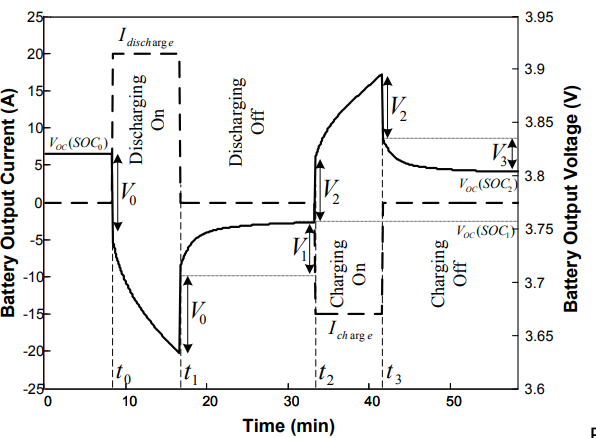
\includegraphics[width=0.5\textwidth]{Chap06/Figures/Batt_Pulsed_current_char.PNG}
	\caption{Characteristic waveforms for battery output voltage and current during charging and discharging of lithium-ion cells.}
	\label{fig:Battery_Current_Pulse}
\end{figure}

\paragraph{Ohmic Resistance :} 
The voltage drop across R0 at the 
first time instant when charging ($V_2$) respectively 
discharging ($V_0$) can be taken to calculate $R_0$ \cite{Internal_Resistance_LIPO_Batt_Gogoana}, according 
to Equation \ref{eq:Batt_Ohmic_Resistance}: 

\begin{equation}\label{eq:Batt_Ohmic_Resistance}
	R_0 =\begin{cases}
	  \frac{V_0}{I_{discharge}}, & \text{: for discharge}.\\
	  \frac{- V_2}{I_{discharge}}, & \text{: for charge}.\\
	\end{cases}
\end{equation}

\paragraph{Estimation of the OTC Model Parameters :} 
in this step 
battery output voltage measurements during the 
subintervals S2 and S4 are used, as in these subintervals 
OCV is constant\cite{Internal_Resistance_LIPO_Batt_Gogoana}, and the battery output voltage is just 
driven by the dynamic characteristics of the battery. The 
output voltage $v_{Batt}$ during S2 and S4 can be calculated 
according to the OTC model by setting $i_{Batt}$ to zero in 
Equations \ref{eq:OTC_Voltage } and \ref{eq:OTC_Batt_Voltage }, then solving the differential equation as 
shown in Equation \ref{eq:Batt_OTC_Diff_Eq_Sol} \cite {UKEMPT_AHMAD2012}:

\begin{equation}\label{eq:Batt_OTC_Diff_Eq_Sol}
	\begin{cases}
	  S_2 : V_{Batt}(t) = V_{OC}(SOC_1) - v_{OTC}(t1) e^{\frac{-t}{\tau_{OTC}}} , & \text{:where,} \tau_{OTC} = R_{OTC}\times C_{OTC}.\\
	  S_4 : V_{Batt}(t) = V_{OC}(SOC_2) - v_{OTC}(t3) e^{\frac{-t}{\tau_{OTC}}}\\
	\end{cases}
\end{equation}

Estimating the values is necessary for the identification of OTC model parameters $V_{OC}(SOC_1),V_{OC}(SOC_2),v_{OTC}(t1),v_{OTC}(t3), \tau_{OTC}$  
in Equations \ref{eq:Batt_OTC_Diff_Eq_Sol}. A nonlinear least squares approach is used (also known as nonlinear data fitting) to find the values that best suit the relationship between the measurements and the nonlinear function, in this case, an exponential function, to estimate these parameters
$f(t) = A + Be^{-\alpha t}$ . \\

The vector of coefficients A, B, and $\alpha$ is the result of the nonlinear least squares algorithm. Through Equations \ref{eq:Batt_OTC_Least_Square_solution} to \ref{eq:Batt_OTC_C_OTC}, these coefficients will be used to calculate the OTC model parameters:

\begin{equation}\label{eq:Batt_OTC_Least_Square_solution}
	\begin{cases}
	  S_2 : V_{OC}(SOC_1) = A, v_{OTC}(t1) = B, & \text{:where,} \tau_{OTC} = \frac{1}{\alpha}.\\
	  S_4 : V_{OC}(SOC_2) = A, v_{OTC}(t2) = B,\\
	\end{cases}
\end{equation}

\begin{equation}\label{eq:Batt_OTC_T_charge_discharge}
	\begin{cases}
		T_{Charge} = t1 - t0\\
		T_{Discharge} = t3 - t2 \\
	\end{cases}
\end{equation}

\begin{equation}\label{eq:Batt_OTC_R_OTC}
	\begin{cases}
	  S_2 : R_{OTC} = \frac{v_{OTC}(t1)}{ \left( 1 - e^{\frac{- T_{Discharge} }{\tau_{OTC} }}\right) I_{Discharge}} \\
	  S_4 : R_{OTC} = \frac{v_{OTC}(t3)}{ \left( 1 - e^{\frac{- T_{Charge} }{\tau_{OTC} }}\right) I_{Charge}} \\
	\end{cases}
\end{equation}

\begin{equation}\label{eq:Batt_OTC_C_OTC}
	C_{OTC} = \frac{\tau_{OTC}}{R_{OTC}}
\end{equation}

\paragraph{Estimation of the TTC Model Parameters :} 

By considering the two RC networks in place of the OTC model's single RC network, the TTC model parameters can be calculated in the same manner as for the OTC model. Equations \ref{eq:Batt_TTC_Diff_Eq_Sol} can be used to define the output voltage of the TTC model for the subintervals S2 and S4. The experiments carried out on the LIPO Battery and the typical parameters of the Battery are shown in table 4.1.

\begin{equation}\label{eq:Batt_TTC_Diff_Eq_Sol}
	\begin{cases}
	  S_2 : V_{Batt}(t) = V_{OC}(SOC_1) - v_{TTC1}(t1) e^{\frac{-t}{\tau_{TTC1}}} - v_{TTC2}(t1) e^{\frac{-t}{\tau_{TTC2}}},&\tau_{TTC1} = R_{TTC1}\times C_{TTC1}.\\
	  S_4 : V_{Batt}(t) = V_{OC}(SOC_2) - v_{TTC1}(t3) e^{\frac{-t}{\tau_{TTC1}}} - v_{TTC2}(t3) e^{\frac{-t}{\tau_{TTC2}}},&\tau_{TTC2} = R_{TTC2}\times C_{TTC2}. \\
	\end{cases}
\end{equation}


\begin{table}[ht]\label{tb:SLPB120216216_Cell_Data }
	\begin{center}
		\begin{tabular}{|c|c|c|}
			\hline
			\multicolumn{2}{|c|}{{Typical Capacity }} & 53 Ah\\
			\hline
			\multicolumn{2}{|c|}{{Nominal Voltage}} & 3.7\\
			\hline
			\multicolumn{1}{|c|}{\multirow{2}{*}{Charge Condition}}& Max. Current & 53A\\ 
			\multicolumn{1}{|c|}{}& Voltage & 4.2V $\frac{+}{-}$ 0.03V\\
			\hline
			\multicolumn{1}{|c|}{\multirow{2}{*}{Discharge Condition}}& Max. Current & 159A\\
			\multicolumn{1}{|c|}{}& Peak Current & 290A\\
			\multicolumn{1}{|c|}{}& Cut-off Voltage & 3.0V\\
			\hline
		\end{tabular}
		\caption{SLPB120216216 Cell Data }
	\end{center}
	\label{tab:multicol}
\end{table}

Estimating the values is required for the TTC model's identification, $V_{OC}(SOC_1), V_{OC}(SOC_2), v_{TTC_1}(t1), v_{TTC_1}(t3), v_{TTC_2}(t1), 
v_{TTC_2}(t3), \tau_{TTC_1}  and  \tau_{TTC_2}$ in Equations \ref{eq:Batt_TTC_Diff_Eq_Sol}. In this 
case an exponential function with two-time constants $f(t)=A+Be^{-\alpha t}+Ce^{- \beta t}$ is used.
\\
The vector of coefficients A, B, C,$\alpha, and \beta$ is the result of the nonlinear least squares algorithm. Through Equations \ref{eq:Batt_OTC_Least_Square_solution} to \ref{eq:Batt_TTC_C_TTC}, these coefficients will be utilized to calculate all the TTC model's parameters. 

\begin{equation}
	\begin{cases}
	  S_2 : V_{OC}(SOC_1) = A 
	  S_4 : V_{OC}(SOC_2) = A
	\end{cases}
\end{equation}

\begin{equation}\label{eq:Batt_OTC_Least_Square_solution}
	\begin{cases}
	  S_2 :  v_{TTC1}(t1) = B, v_{TTC2}(t1) = C ,& \text{:} \tau_{TTC1} = \frac{1}{\alpha}.\\
	  S_4 :  v_{TTC1}(t3) = B, v_{TTC2}(t3) = C ,& \text{:} \tau_{TTC2} = \frac{1}{\beta}.\\
	\end{cases}
\end{equation}

\begin{equation}\label{eq:Batt_TTC_R_TTC1}
	\begin{cases}
	  S_2 : R_{TTC1} = \frac{v_{TTC1}(t1)}{ \left( 1 - e^{\frac{- T_{Discharge} }{\tau_{TTC1} }}\right) I_{Discharge}} \\
	  S_4 : R_{TTC1} = \frac{v_{TTC1}(t3)}{ \left( 1 - e^{\frac{- T_{Charge} }{\tau_{TTC1} }}\right) I_{Charge}} \\
	\end{cases}
\end{equation}

\begin{equation}\label{eq:Batt_TTC_R_TTC2}
	\begin{cases}
	  S_2 : R_{TTC2} = \frac{v_{TTC2}(t1)}{ \left( 1 - e^{\frac{- T_{Discharge} }{\tau_{TTC2} }}\right) I_{Discharge}} \\
	  S_4 : R_{TTC2} = \frac{v_{TTC2}(t3)}{ \left( 1 - e^{\frac{- T_{Charge} }{\tau_{TTC2} }}\right) I_{Charge}} \\
	\end{cases}
\end{equation}

\begin{equation}\label{eq:Batt_TTC_C_TTC}
	\begin{cases}
		C_{TTC1} = \frac{\tau_{TTC1}}{R_{TTC1}} \\
		C_{TTC2} = \frac{\tau_{TTC2}}{R_{TTC2}} \\
	\end{cases}
\end{equation}

\subsection{Experimental and Computational Results of SLPB120216216}
Cells made of lithium polymer by the producer Kokam were employed for the modeling and experimental experiments.
Table 4.1 shows several significant cell data. A battery test bench was established to determine the model parameters. Using short and long interruptions, a rectangular-shaped current signal must be applied to the battery on this test bench. It is also necessary to measure the voltage of the battery output. While the OTC and TTC model parameters must be determined during extended pauses, the battery's ohmic resistance R0 can be measured during small interruptions of the current signal.

\begin{figure}[h]
	\centering
	\subfigure[Ohmic Resistance $R_0 = f(SOC) @ Discharging $]{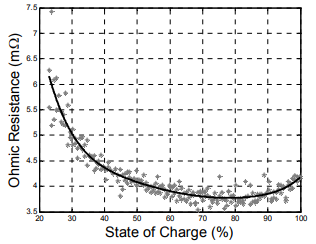
\includegraphics[scale=.8]{Chap06/Figures/Batt_DisCh_Ohmic_Resistance.PNG}}
	\qquad
	\subfigure[Ohmic Resistance $R_0 = f(SOC) @ Chareging $]{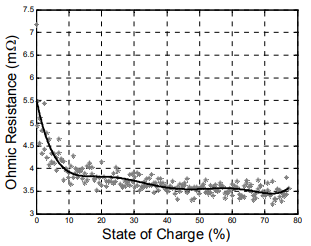
\includegraphics[scale=.8]{Chap06/Figures/Batt_Ch_Ohmic_Resistance.PNG}}
	\qquad
	\subfigure[Output Voltage of the Battery $@ Discharing$]{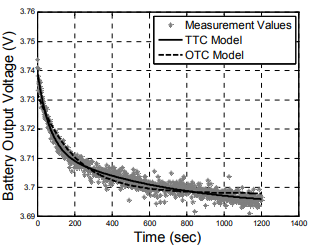
\includegraphics[scale=.8]{Chap06/Figures/Batt_DisCh_OutPut_Voltage.PNG}}
	\qquad
	\subfigure[Output Voltage of the Battery $@ Charging $]{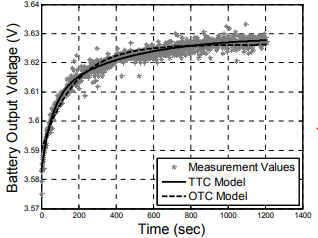
\includegraphics[scale=.8]{Chap06/Figures/Batt_Ch_OutPut_Voltage.PNG}}
	\qquad
	\subfigure[Dynamic Resistance of the Battery  $R_{OTC}/R_{TTC1}/R_{TTC_2} = f(SOC) @ Discharging $]{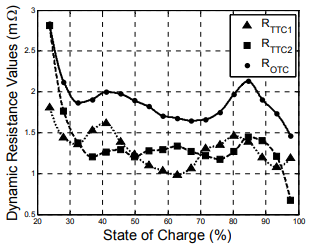
\includegraphics[scale=.8]{Chap06/Figures/Batt_DisCh_Resistance.PNG}}
	\qquad
	\subfigure[Dynamic Resistance of the Battery $R_{OTC}/R_{TTC1}/R_{TTC_2} = f(SOC) @ Charging $]{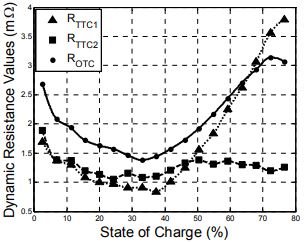
\includegraphics[scale=.8]{Chap06/Figures/Batt_Ch_Resistance.PNG}}
	\qquad
	\subfigure[Dynamic Capacitance of the Battery  $C_{OTC}/C_{TTC1}/C_{TTC_2} = f(SOC) @ Discharging $]{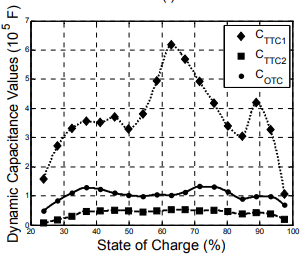
\includegraphics[scale=.8]{Chap06/Figures/Batt_DisCh_Capacitance.PNG}}
	\qquad
	\subfigure[Dynamic Capacitance of the Battery $ C_{OTC}/C_{TTC1}/C_{TTC_2} = f(SOC)  @ Charging $]{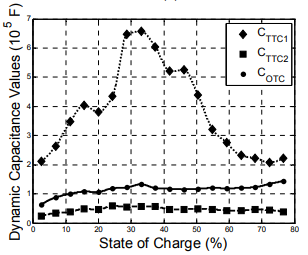
\includegraphics[scale=.8]{Chap06/Figures/Batt_Ch_Capacitance.PNG}}
	\caption{LIPo Battery SLPB120216216 Simulated Results \cite{UKEMPT_AHMAD2012} }
	\label{fig:LIPO_Batt_SLPB120216216_Results}
\end{figure}
  
\section{Battery Emulation}

\textit{Part I} of the chapter \ref{ch:Battery_Modeling_Emulation} described extensively the LIPO Battery Modeling and equivalent circuit analysis. The \textit{Part II} of the chapter gives more extravagance to the Battery model implemented in real-time. \textit{Part II} will also talk about different instrumentation and configurations. I have used and python environment to implement the system, the reason behind choosing python as a coding environment is, python is a high-level used and most compatible with different instruments. The basis for implementing the battery model is the data that is collected for the SLPB120216216 by Ahmad RAHMOUN, Helmuth BIECHL. Gratitude to \textit{Ahmad RAHMOUN and Helmuth BIECHL} for their paper\cite{UKEMPT_AHMAD2012} \textit{"Modelling of Li-ion batteries using equivalent circuit diagrams"} this paper became the bedrock for this module implementation. Following the upcoming sections is the continuation of the \textit{Part I} battery modeling with the coding environment.

\begin{figure}[h]
	\centering
	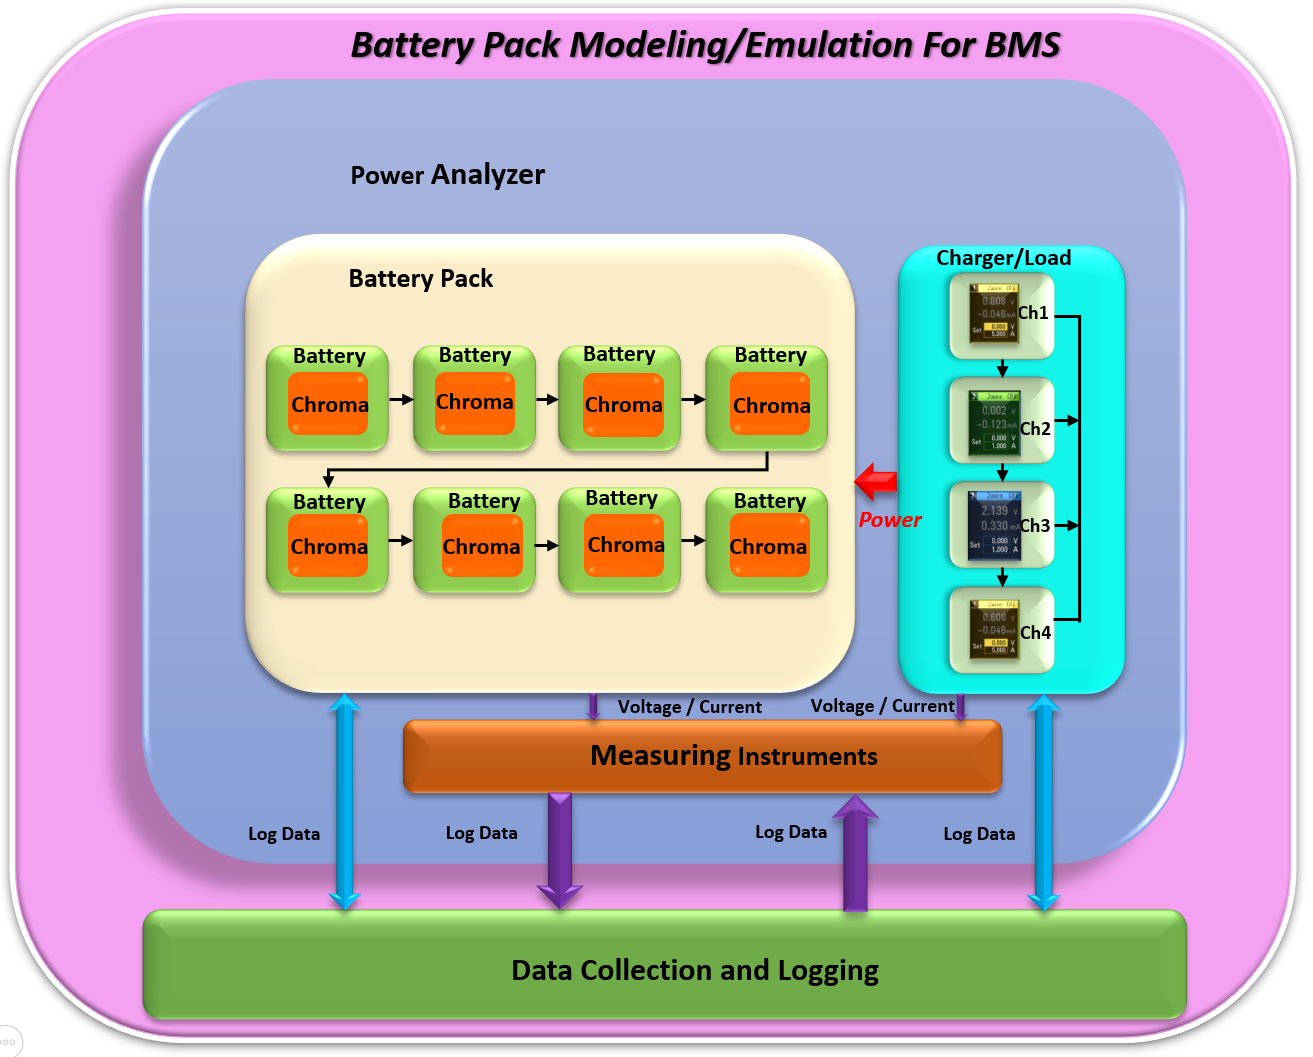
\includegraphics[width=0.9\textwidth]{Chap06/Figures/Battery_Pack_modeling_Architec.PNG}
	\caption{Architecture of the Battery Pack Modeling/Emulation For BMS}
	\label{fig:Battery_Pack_modeling_Architec}
\end{figure}

\subsection{Fundamental Instruments For Battery Emulation }

Figure \ref{fig:Battery_Pack_modeling_Architec} shows the architecture of the Battery modeling and the emulation, for the external view the architecture looks very clumsy and dusky, but I have followed the modular approach in this architecture to extend the model to a one-time constant or two-time constant even three. The proposed architecture can handle multiple current sourcing, sinking, and measuring instruments without disturbing the overall system. Before diving into the architecture and modular approach, it is good to understand what kind of instruments can be used. And their specifications for the BMS applications. The following section can give brief information on the instruments and their configurations.

\subsubsection{Chroma :}
% \begin{figure}[h]
% 	\centering
% 	\subfigure[16CH Battery Cell Simulator 87001]{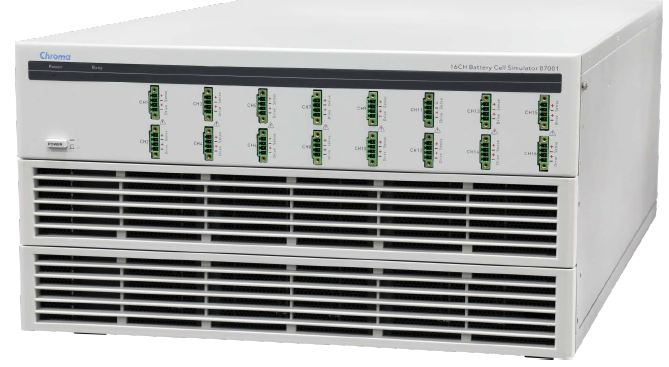
\includegraphics[width=0.4\textwidth]{Chap06/Figures/Chroma.PNG}}
%     \qquad
% 	\subfigure[Chroma Output Wiring to the BMS]{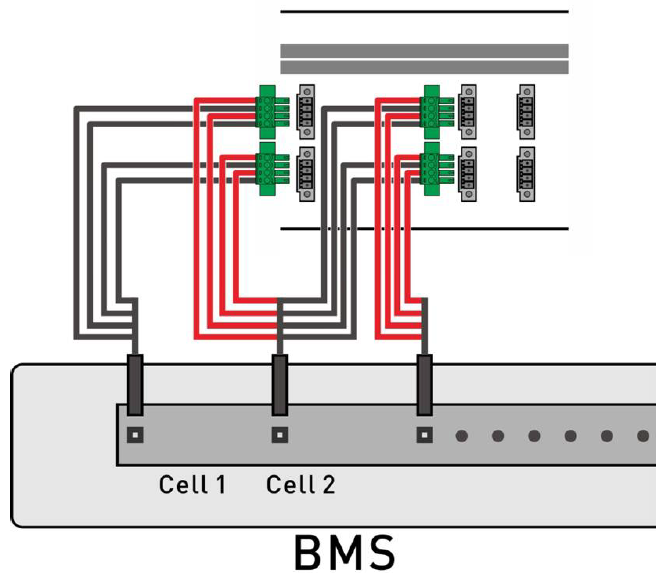
\includegraphics[width=0.4\textwidth]{Chap06/Figures/Chroma_Output_wiring.PNG}}
% 	\caption{16CH Battery Cell Simulator 87001}
% 	\label{fig:Chroma}
% \end{figure}
The 87001 16CH Battery Cell Simulator can simulate the cell to perform charge and discharge behavior for BMS testing. It can simulate up to 480 battery cells in series with voltage and current measurement functions. It can receive IPC's commands in real-time, store the measured values temporarily and return them to the IPC \cite{Chroma_UserManual}.Chroma has two communication one through the ethernet and CAN bus, for facilitating the modular and easy communication I preferred ethernet for this particular project, we can also use the can bus when we test the emulator with the real-time vehicle setup. Figure \ref{fig:Chroma}(a) shows the 16CH chroma which I have used in the lab.

\paragraph{Sepcifications of the Chroma :}

\begin{itemize}
    \item This simulator has built a DC Power Supply with 1Φ110~220V±10$\%$VLN input power.
    \item Each unit has 16 channels output that can set parameters, start and end time respectively.
    \item The channel can be a constant voltage source with a constant current function.
    \item Maximum 30 sets of 87001 simulators can be connected in series for use and can simulate the battery cell voltage of a 480-cell battery pack (2000V/4.2V) in series.
    \item High-precision output and measurement that are used in laboratories for testing product specifications and characteristics.
    \item No display panel and operation buttons but using LED lights to indicate the standalone unit status.
    \item Each channel has 2 current ranges (2 Current: (-5A~+5A, -0.5A~+0.5A) ).
    \item The operating interface uses the internet to give commands, control output measurement and read data via an external PC. The communication interface is Ethernet with SCPI protocol specification.
    \item Channels can be connected in series/parallel across a standalone unit with up to two batteries connected in parallel.
    \item Noise < 60db (output terminal 5V/5A/16CH)
    \item \textbf{Auto Range Select }
            \begin{itemize}
                \item The CC automatically switches to the proper range according to the set current.
                \item The CV automatically switches to the mapping range according to the upper limit current.
            \end{itemize} \ref{fig:Chroma}(a)
    \item \textbf{Current Range Select }
            \begin{itemize}
                \item When 5A is in use, performing CC(Constant Current) charge for 500uA may have a bigger error.
                \item When 500mA is in use, performing CC charge for 5A will prompt a warning and stop execution.
            \end{itemize}

    \item \textbf{Data Transmission :} The data transmission interval is 10ms * paralleled unit no. The minimum data transmission interval is Δ10ms for one unit and Δ20ms for two units, and so forth.
    
\end{itemize}

\paragraph{Output Wiring of the Chroma :}
% \begin{figure}[h]
% 	\centering
% 	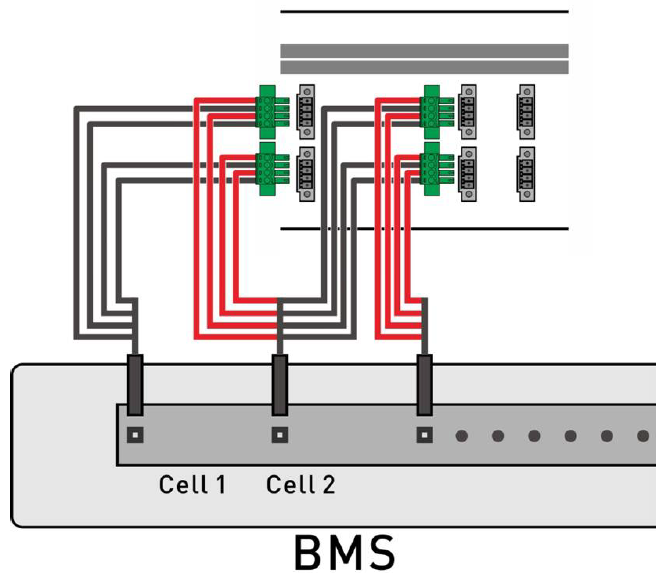
\includegraphics[width=0.4\textwidth]{Chap06/Figures/Chroma_Output_wiring.PNG}
% 	\caption{Chroma Output Wiring to the BMS} 
% 	\label{fig:Chroma_Output_wiring}
% \end{figure}

\begin{itemize}
    \item The figure \ref{fig:Chroma}(b) is the parallel connection diagram of two simulators \cite{Chroma_UserManual}. (Same for serial connection.)
    \item The 87001 is a 4-wire measurement. The SENSE wire and BMS connection point should be as close as possible to the BMS input terminal to avoid voltage differences due to line losses.
\end{itemize}

\paragraph{Configuring the Chroma:}

For Programing the Chroma I took the help of the pyvisa library, which can use to interface with instruments using different protocols. The first setup is the NI (National Instrument) driver in PC to identify the instrument (install NI Max application in PC), through the NI driver, pyvisa can communicate through the VISA virtual port. The piece of code shows how to configure the visa port for the chroma(or any battery emulator commands that are more generalized) \cite{Chroma_UserManual}.

% \lstinputlisting[language=python]{Chap06/Code/Chroma.py}
\begin{lstlisting}[language=Python, caption=VISA parameters set for Chroma]
    #VISA commands for the Chroma
    set_visa_attribute(pyvisa.constants.VI_ATTR_MAX_QUEUE_LENGTH, 50)
    #Time Out Value 
    set_visa_attribute(pyvisa.constants.VI_ATTR_TMO_VALUE, 2000) 
    set_visa_attribute(pyvisa.constants.VI_ATTR_TERMCHAR_EN, 
                        pyvisa.constants.VI_TRUE)
    set_visa_attribute(pyvisa.constants.VI_ATTR_TERMCHAR, 0xA) 
    set_visa_attribute(pyvisa.constants.VI_ATTR_SEND_END_EN, 
                       pyvisa.constants.VI_TRUE) 
    
    set_visa_attribute(pyvisa.constants.VI_ATTR_SUPPRESS_END_EN, 
                       pyvisa.constants.VI_TRUE)
    set_visa_attribute(pyvisa.constants.VI_ATTR_FILE_APPEND_EN, 
                       pyvisa.constants.VI_FALSE) 
    set_visa_attribute(pyvisa.constants.VI_ATTR_IO_PROT, 1) 
    set_visa_attribute(pyvisa.constants.VI_ATTR_TCPIP_NODELAY, 
                       pyvisa.constants.VI_TRUE) 
    set_visa_attribute(pyvisa.constants.VI_ATTR_TCPIP_KEEPALIVE, 
                       pyvisa.constants.VI_TRUE)
\end{lstlisting}

The following code explores the basic programming of the chroma for BMS application:

\begin{lstlisting}[language=Python, caption=Basic BMS Program for Chroma]
    #Basic Program for Chroma to configure the cells
    chroma.query('*IDN?\n') # identify the instrument
    #Query the output sampling time
    chroma.query('SIM:CONF:SAMP:TIME?\n') 

    #number of BMS(each Chroma is One BMS) are parallel
    chroma.write(f'SYST:SLAVE:PARA {self.noOfBMS}\n')
    chroma.write(f'SYST:SLAVE:SCAN {self.noOfBMS}\n')

    #Chroma Status commands
    chroma.query('SYSTem:FRAME:STATe? 0\n')
    chroma.query('SYST:FRAME:CHAN:STATe? 1\n')
    chroma.query('SYST:FRAME:CHAN:NUMB? 0\n')
    chroma.write('SIM:CONF:CHAN:ACT 65535\n')
    chroma.write('SIM:CONF:CLE\n'

    ''' BMS configurations '''
    #Number of the BMS 1
    chroma.write(f'SIM:CONF:BMS:NUMB {noOfBMS}\n')
    #No cells use in the BMS testing #1 BMS , #2 Cells 
    chroma.write(f'SIM:CONF:CELL:NUMB {noOfBMS},{noOfBMSCells}\n')
    #BMS 1, CellStart 1, Cellend 2, 
    # Cell parallel to the channel1 , # Current Range 2  - 5.0 A
    chroma.write(f'SIM:CONF:CELL:PARA {noOfBMS},{noOfBMS},
    {noOfBMStestingCells},{paralleBMSchannel},{cellCurrent_5A}\n') 

    ''' Output Parameters Set '''

    ''' # BMS start  1 ,# BMS end 1 ,#set the start cell 1, 
    # set the end cell 1, # set the cell voltage 4.0 ,
     # set the Current of the cell 0.5A '''

    chroma.write(f'SIM:PROG:CELL {noOfBMS},{noOfBMS},{cellNo},
    {cellNo},{cellVoltage},{cellCurrent5A}\n') 

    # Switch on all the cells immediately
    chroma.write('SIM:OUTP:IMM\n') 

    '''### check if there is any error 
    in the Chroma while setting the voltages 
    ### if there is no error enable
     all the cells outputs''' 

    time.sleep(10)
    # Check the configuration Error 
    self.chroma.query('SYST:ERR?\n')

    # Switch on all the cells
    self.chroma.write('SIM:OUTP ON \n')  
    time.sleep(1) # give some time to switch on the emulator 

\end{lstlisting}

The above-attached code is just a basic code for the BMS application which can give a better idea about the basic chroma(Battery emulator) for more SCPI commands of the chroma follow the user manual\cite{Chroma_UserManual} and for the detailed class-based skeleton follow \textcolor{blue}{here}. %\href{}{here}.

\paragraph{Response Time of the Chroma :}
During battery, balancing it is essential to capture the battery voltage, in reality, this is not the problem because we might be dealing with the actual batteries which do not need voltage updates to the batteries. When we deal with any instruments (battery emulators) it is essential to update the battery (Cell) voltages and battery currents. In this particular project, chroma is used as the battery emulator. Chroma is being communicated through a python script to update its parameters via ethernet. The fundamental response time of the chroma for every request is 10ms, that being said for our application few 100ms time duration is good enough for calculating the batteries SoC. Perhaps I made some demonstration of the chroma response time and the number of packets, figure \ref{fig:Chroma_Packet_delay} shows the round robbin delay of 8 cells current and voltage fetch from chroma.
The results are quite adequate, over 10k packet request chroma has missed one or two chances of delaying 500ms, which still satisfies a few million packets.

\begin{figure}[h]
	\centering
	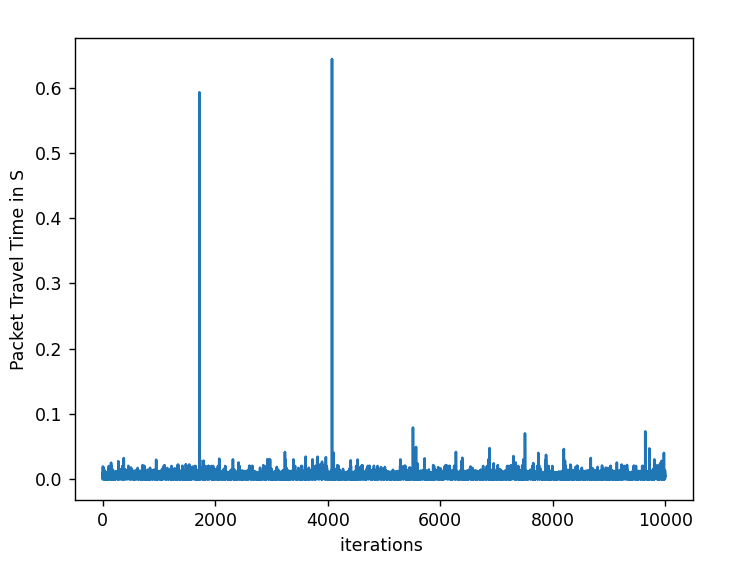
\includegraphics[width=0.5\textwidth]{Chap06/Figures/Chroma_Packet_delay.png}
	\caption{Chroma Response Time for Voltage and Current Request }
	\label{fig:Chroma_Packet_delay}
\end{figure}

\subsubsection{Load/Charger :}

In the setup\ref{fig:Battery_Pack_modeling_Architec} load or charger is used across the series cells (battery pack) which can only supply current or sink current from the pack. For this particular architecture, I have preferred e Keysight N6705 DC Power Analyze as a load or charger. All the controls have been passed through the power analyzer module through the script.

\paragraph{ Keysight N6705 DC Power Analyzer :}

The Keysight N6705 Figure \ref{fig:keysight_n6705_DMM_34460A}(a) DC Power Analyzer is a multipurpose power system that combines the capabilities of an oscilloscope, a data logger, and a DC voltage source with numerous outputs \cite{Keysight_N6705_DC_Power_Analyzer}.

The Keysight N6705 has up to four programmable outputs as a multiple-output DC source. The power levels of the available power modules range from 20 W to 500 W, with different voltage and current combinations, and they offer a wide range of performance capabilities. Additionally, each output can generate arbitrary (Arb) waveforms, allowing you to program. Standardized voltage and current waveforms, or create your own. With Keysight N678xA SMUs (Source/Measure Units) have a multi-quadrant power mesh with distinct voltage and sources of current priority \cite{Keysight_N6705_DC_Power_Analyzer}.

% \begin{figure}[h]
% 	\centering
% 	\subfigure[4 Channel keysight N6705 Power Supply]{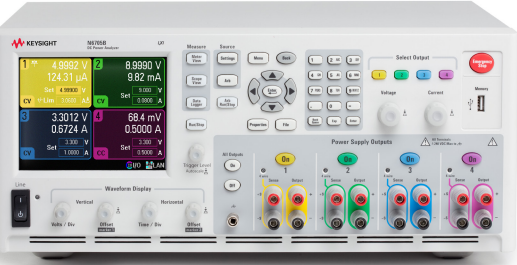
\includegraphics[width=0.4\textwidth]{Chap06/Figures/keysight_n6705.PNG}}
%     \qquad
% 	\subfigure[Chroma Output Wiring to the BMS]{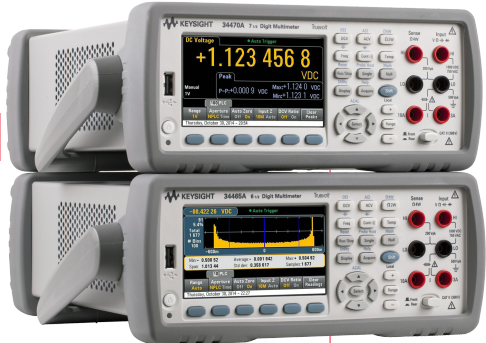
\includegraphics[width=0.4\textwidth]{Chap06/Figures/DMM_34460A.PNG}}
% 	\caption{ keysight N6705 Power Supply and DMM 34460A }
% 	\label{fig:keysight_n6705_DMM_34460A}
% \end{figure}

The Keysight N6705's Meter View shows the average output voltage and current as a measurement system. Scope View, which you can modify using the vertical and horizontal sliders, displays waveforms. The Data Logger View records average and peak voltage and current measurements over a long period and plots the data \cite{Keysight_N6705_DC_Power_Analyzer}.

The setup allows configuring the DC power supply as a charger or load, by setting the current direction.  The following program shows the typical program for load/chargers:

\begin{lstlisting}[language=Python, caption=Load/Charger Configuration for Keysight N6705's]

    #find the resource
    rm = pyvisa.ResourceManager()
    #open the instrument by the id 
    loadCh = rm.open_resource('USB0::0x0957::0x0F07:
                    :MY50000622::INSTR')
    #Identify Keysight N6705's
    loadCh.query('*IDN?\n')
    
    '''Configure Power analyzer channels 1 and 3 in 
    2 quadrants to sink or source current; that presumes 
    Load or Charger'''
    loadCh.write('EMUL PS2Q,(@1,3)')

    # Eneable current priority for channels 1 and 3
    loadCh.write('FUNC CURR,(@1,3)')
    
    # Set currnet range for 1 and 3 channel  1Amp
    loadCh.write('SOUR:CURR:RANG 1.02,(@1,3)')
    loadCh.write('CURR 1,(@1,3)')
    
    #Set Voltage limt for 28V
    loadCh.write('VOLT:LIM 28,(@1,3)')

    # Switch on Channel 1 and channel 3
    loadCh.write('OUTP ON,(@1,3)')
    
\end{lstlisting}

The above program is just an example of programming channel 1 and channel 3, we can couple the power supply channels for programming and trigger at the same time ($OUTP:COUP:CHAN$ \textit{1,2 ; Couple channel 1 and 2}). For more details and programming examples, refer to the keysight N6705B datasheet \cite{Keysight_N6705_DC_Power_Analyzer}.

\subsubsection{Meter View :}
The proposed architecture \ref{fig:Battery_Pack_modeling_Architec} encounters a meter view, which meter view allows the collaboration of various measuring instruments which can be directly controlled. A meter view in the architecture is directly controlled by the power analyzer module. Measurements include DC/DC converter input/output current measurements, and battery pack current measurements. The current measurement setup in the system is very much critical, hence we can measure the shunt voltage, and we can calculate the current flow (if shunt resistance is known). Measurement view is so much modular that we can have as many measuring instruments in the setup, and we log the data without disturbing the setup.
In the architecture, keysight 34470A DMM  \ref{fig:keysight_n6705_DMM_34460A}(b) has been employed for shunt voltage measurements (Battery Pack Current, DC/DC input/output current; Fig \ref{fig:BMS Architecture}). The following sections will give more detailed information about the multimeter and configuration.

\paragraph{Digital Multimeters 34460A :}

% \begin{figure}[h]
% 	\centering
% 	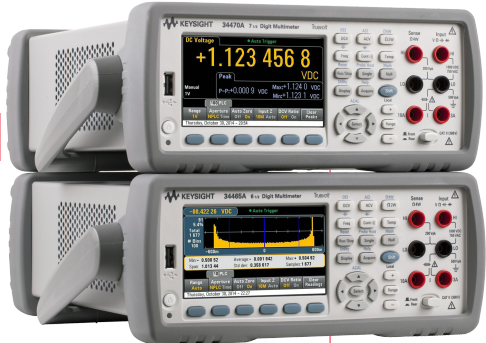
\includegraphics[width=0.4\textwidth]{Chap06/Figures/DMM_34460A.PNG}
% 	\caption{Keysight Technologies Digital Multimeters 34460A}
% 	\label{fig:keysight_DMM_34460A}
% \end{figure}

The only completely drop-in, SCPI-compatible alternative to the 34401A DMM in the market is the Digital Multimeters 34461A \cite{Keysight_34460A_DMM}. Although some other DMMs claim to be 34401A SCPI compatible, they only support a limited number of SCPI commands. The same design team that produced the 34401A also produced the Truevolt DMMs. When developing the Truevolt family of DMMs, the team kept 34401A measures, dependability, and familiarity in mind. Consequently, people may use it without having to spend hours learning how.
The following basic programming for DMM gives more insights into communication and configuration for measurement setup :

\begin{lstlisting}[language=Python, caption=DMM Keysight 34401A's Meauring/Configuration ]
    rm = visa.ResourceManager()
    ''' usb_id='USB0::0x2A8D::0x1301::MY57216238::INSTR' VISA id of DMM 
    Open VISA port
    '''
    mul_34461A = rm.open_resource(usb_id)

    #Identify DMM
    mul_34461A.query('*IDN?')
    #Rest DMM
    mul_34461A.write('*RST')
    #Check for Error
    mul_34461A.query('SYST:ERR?')  
    # set NPLC to speed up the measurements
    mul_34461A.write('VOLT:DC:NPLC 0.02')  

    ''' Configure DMM for Voltage measurements '''
    mul_34461A.write(':FUNC "VOLT:DC"') 
    if range in range_list:
            range_auto = ':VOLT:DC:RANG:AUTO '
            range_val = ';:VOLT:DC:RANG '
            res_com = ';:VOLT:DC:RES '

            if range == -1:
                range_auto_cmd = 'ON'
                range_val = ''
                range_val_str = ''
                res_com = ''
                res_val_str = ''
            else:
                range_auto_cmd = 'OFF'
                range_val_str = str(range)
                if range == 0.1 or range == 1:
                    res = 1e-6
                elif range == 10:
                    res = 1e-5
                elif range == 100:
                    res = 1e-4    
                else:   
                    res = 1e-3
                res_val_str = str(res)

            com = range_auto + range_auto_cmd +  range_val + 
            range_val_str + res_com + res_val_str

            #wite the Command
            mul_34461A.write(com) 
            mul_34461A.write('VOLT:IMP:AUTO ON')
            array = []
            while count>0:
                if count > 4:
                    cnt = 4
                else:
                    cnt = count 
                array.append(self.read_value(cnt))
                count -= 4 
            return(sum(array)/len(array))   
        else:
            return('ERR: Wrong range')   

    # Fetch the voltage 
    def Volt(self):
        return float(mul_34461A.query('READ?')) 
\end{lstlisting}

\subsection{ Battery Modeling :}
The above sections have described the hardware and instrument setup in the Battery Emulation architecture \ref{fig:Battery_Pack_modeling_Architec}. After understanding the background and programming setup for instruments it is easy to understand the Battery modeling algorithms. The following sections can discretize the Battery emulation architecture and explain the algorithms.

\begin{algorithm}[H]\label{algo:Battery_Modeling}
    \DontPrintSemicolon
    \SetAlgoLined
    \KwData{$BattModel$ = $<Q_{tot},dt,SOC_0,V_{batt},V_{oc},SoC,i_{batt},BattModelParams(SoC)>$}
    \SetKwInOut{Input}{input}\SetKwInOut{Output}{output}
    \Input{$Q_{tot}$,  $dt$ , $SOC_0$ }
    \Output{$V_{batt}$,$V_{OTC_(k+1)}$,$SOC$}
    Initialization\;

        $Q_{tot} \leftarrow$ Total Batt Capacity $\mathcal{N})$(0.1 ~ 100) Ah\\
        $SOC_0 \leftarrow$ Initial SoC ($SoC_{(k)})$ $\mathcal{N}$ (0 ~ 1) \\
        $dt \leftarrow$  Measurement Sampling time $\mathcal{N}$(0 ~ 1000) mS \\   
        $i_{batt} \leftarrow$ = 0 ; initial battery current $i_{batt(k)}$\\  
        $V_{OC(k)}   = BattModelParams.VOC(SoC_{(k)})$ \CommentSty{BatteryOpen ckt Voltage $ f(SoC_0)$}\\
        \For{k $\leftarrow 0$ \KwTo iters}{
            $R_{0(k)} = BattModelParams(SoC_{(k)})$\\
            $C_{OTC(k)} = BattModelParams.COTC(SoC_{(k)})$\\
            $R_{OTC(k)} = BattModelParams.ROTC(SoC_{(k)})$ \CommentSty{Battery OTC Dynamic Components $ f(SoC)$}\\
            $V_{OC(k)}   = BattModelParams.VOC(SoC_{(k)})$ \CommentSty{BatteryOpen ckt Voltage $ f(SoC)$}\\
            $V_{batt(k)} = V_{OC(k)} - V_{OTC(k)} - R_0(k)\times i_{batt(k)}$\\
            $V_{OTC(k+1)} = V_{OTC(k)} \times exp^{ \frac{- dt} { C_{OTC(k)} * R_{OTC(k)} }} +  R_{OTC(k)}\times ( 1 - exp^{ \frac{- dt} { C_{OTC(k)} * R_{OTC(k)} }})\times i_{batt(k)}$\\
            $SoC(k+1) = SoC(k) - i_{batt(k)}\times \frac{dt} {Q_{tot} * 3600}$ \CommentSty{Coloumb SOC}\\
            $i_{batt(k+1)} \leftarrow$  $i_{battNew}$ \CommentSty{the latest Battery current measurement}\\

            }
    \Return{$V_{batt(k)},SoC_{(k)},V_{OTC(k+1)} $}\\
    \caption{Battery Modeling Algorithm}
\end{algorithm}


The section shows the basic battery modeling algorithm, the explanation is as follows:
\begin{equation}\label{eq:coulomb_soc}
    SoC(k+1) =  SoC(k)  \pm dt\times \frac{i_{batt(k)}}{Q_{tot}}
\end{equation}
\begin{itemize}
    \item $Batt$ module name which will take  $<Q_{tot},dt,SOC_0,i_{batt},BattModelParams(SoC)>$ inputs and produces $V_{batt},V_{OC},SoC>$ as the outputs
    \item Initialization of the algorithm parameters
    \begin{itemize}
        \item $<Q_{tot}$ is the total capacity of the battery and $dt$ measurement time used to calculate the battery SoC for instance by the coulomb count eq :\ref{eq:coulomb_soc}
        \item $SOC_0$ initial SoC which can help to extract the open circuit voltage($V_{OC}$) of the battery at first instance, when $i_{Batt}$ = 0 the $V_{OC}$ is same as $V_{Batt}$
        \item Open circuit voltage($V_{OC}$) is the function of the SoC, the $V_{OC}$ can directly extract from the Battery Voltage/SoC curve which will be provided by the battery manufacturer 
        \item $BattModelParams(SoC)$ module take SoC as input provide the Battery modeling parameters $V_{OC},R_0,C_{OTC},R_{OTC}$ by interpolating SoC with the manufacturer provided battery component lookup tables 
    \end{itemize}
    \item Iterate the for (k) loop  from 0 to N -1
    \item For every $SoC(k)$ $BattModelParams(SoC_{(k)})$ will provide $k^{th}$ updated batter parameters $V_{OC(k)},R_{0(k)},C_{OTC(k)},R_{OTC(k)}$
    \item Battery voltage is calculated by the equation \ref{eq:Discrete_eOTC_Batt_Voltage } ; initial $V_{OTC}$ = 0 , $\because i_{batt} = 0$ 
    \item The updated onetime constant voltage of the battery $V_{OTC(k+1)}$ is calculated by the equation \ref{eq:Discrete_OTC_Voltage }
    \item Update the $SOC_(k+1)$ by any SoC calculating algorithms for instance Coulomb count \ref{eq:coulomb_soc} or Kalman etc
    \item The battery current $i_{batt}$ updated with the latest current acquisition made in $dt$ delay 
    \item $Batt$ module will return updated {$V_{batt(k)},SoC_{(k+1)},V_{OTC(k+1)} $} battery voltages and SOC
\end{itemize}

\subsection{Battery Pack Modeling :}
The battery pack module will instantiate the $BattModel$ \ref{algo:Battery_Modeling}, a module created in algorithm \ref{algo:Battery_Pack_Modeling}  which will manage several batteries depending on the user's requirements(setting the updated battery voltages, calculating SoC, measuring batteries current). The algorithm describes the implementation of the battery pack for 8 batteries, we can extend even further just by changing the initial SoC array for the module.
\begin{algorithm}[H]\label{algo:Battery_Pack_Modeling}   
\DontPrintSemicolon
    \SetAlgoLined
    \KwData{$BattPack$ = $<Q_{tot},dt,N_{Batts},SOC_0[] ,V_{batt}[],V_{oc}[],SOC[],i_{batt}[],$
                        $BattModel(), Chroma(V_{Batt})[]>$}

    \SetKwInOut{Input}{input}\SetKwInOut{Output}{output}
    \Input{$Q_{tot}$,  $dt$ , $SOC_0[]$ }
    \Output{$V_{batt}[]$,$SOC[]$}
    Initialization\;
    $Q_{tot} \leftarrow$ Total Batt Capacity  $\mathcal{N} $(0.1 $\sim $ 100) Ah\\
    $SOC_0[] \leftarrow$ Initial SoC ($SoC_{(k)}[]$) $\mathcal{N}$ [1 $\cdots$  8] (0 $\sim $ 1) \\
    $N_{Batts} = len(SOC_0[])$ \CommentSty{No of Cells in BATT Pack}\\
    $dt \leftarrow$  Measurement Sampling time $\mathcal{N}$(0 $\sim $ 1000) mS \\   
    $i_{batt}[] \leftarrow$ = 0 ; initial battery current $i_{batt(k)}$ [1  $\cdots$ $N_{Batts}$]\\  
    $Batt = []$ \CommentSty{Store $BattModel()$ instances}

    \CommentSty{Initialize Chroma Channels}\\
    $Chroma(V_{Cell}=default (4V),N_{Batts} )$

    \CommentSty{Initialize $N_{Batts}$ Battery Model instances\\
        with $SoC_0$
    }\\
    \For{i $\leftarrow 0$ \KwTo $N_{Batts} - 1$}{
        $Batt[i] = BattModel(SOC_0[i] ,Q_{tot},dt)$
    }

    \For{k $\leftarrow 0$ \KwTo $N_{Batts}$}{
        $i_{batt}[k] \leftarrow = Chroma.Currents[k]$ \\
        $[V_{batt}[k],V_{oc}[k]] = Batt[k].battVoltage(i_{batt}[k])$\\
        $SoC[k] = Batt[k].CoulombSOC()$
        $Chroma.VoltageSet(cellNo=k,V_{Cell}=V_{OC}[k])$
    }
    \Return{$V_{batt}[], SOC[] $}\\
    \caption{Battery Pack Modeling Algorithm}
\end{algorithm}

\begin{itemize}
    \item The battery pack module will operate everything on batch-wise like Soc, current, and voltage as arrays ($SOC_0[] ,V_{batt}[],V_{oc}[],SOC[],i_{batt}[]$).
    \item Initialize $Q_{tot},dt , SoC_0[]$ is the initial soc of the batteries which can be declared as an array the length $N_{Batt} = len(SoC_0[])$ of the array determines the number of batteries used in the battery pack.
    \item $i_{batt}[] = 0$ array initialized to zero because there is no current flow at t=0, and declare  $Batt[] = len([],N_{Batt})$ empty array of $N_{Batt}$ size to store the BatteryModel module instance, each instance will operate individually as a battery.
    \item Initialize and configure chroma for $N_{Batt}$ channels in series with an initial voltage of 4v and a maximum current of 5A  $Chroma(V_{Cell}=default (4V),N_{Batts} )$.
    \item Collect the $N_{Batt}$ Battery Model instance in the Batt array;  each  Battery Model module will take initial parameters $SoC_0, Q_{tot} and dt$ as inputs.
    \item Iterate for (k) loop 0 to $N_{Batt} -1$ to emulate each battery from $Batt[k]$ instances
        \begin{itemize}
            \item Measure $i_{batt}[k]$ of $k^{th}$ battery from chroma; $Chroma.Currents[k]$ can provide the current flowing in the $k^{th}$ of the chroma
            \item $k^{th}$ battery model instance function $Batt[k].battVoltage(i_{batt}[k])$ newly calculated battery voltage and $SoC(k)$ corresponding open circuit voltage $V_{OC}$
            \item $SoC[k] = Batt[k].CoulombSOC()$ will calculate the updated SoC by the newly acquired $i_{batt}(k)$
            \item Set the $k^{th}$ battery/channel voltage of the chroma to newly estimated $V_{OC}$
        \end{itemize}
    \item The loop will return  $N_{Batt}$ batteries updated $SOC[]$ and $V_{batt}[]$
\end{itemize}

\subsection{Power Analyzer Modeling}
\begin{algorithm}[H]\label{algo:PowerAnalyzer_Modeling}
    \DontPrintSemicolon
    \SetAlgoLined
    \KwData{$PowerAnalyzer$ = $<BattPack(), LoadCharger() , MeterView() , DataCollection(),dt, SOC[] , V_{Batt}[]>$}
    \SetKwInOut{Input}{input}\SetKwInOut{Output}{output}
    \Input{$BatteryPack(), LoadCharger() , MeterView()$ }
    \Output{$SOC[] , V_{Batt}[]$}
    Initialization all the instruments with VISA USB id\;
    $dt \leftarrow$  Measurement Sampling time $\mathcal{N}$(0 $\sim $ 1000) mS \\   
    $battPack = BattPack()$; $loadCharger = LoadCharger()$; $meterView = MeterView()$ \\
    $BattLowV = 2.5 ; Volts$; $BattHighV = 4.2; Volts$ \\
    $DCDCShunt$ = 3$e^{-3}$ ; $\Omega$; $PackShunt$ = 500$e^{-6}$ ; $\Omega$\\
    $SOC[] = [] , V_{Batt}[] = []$ \\
    \CommentSty{ Tigger DC/DC Converter}\\
    $meterView.Digilent.TriggerDCDC()$\\
    \While{$TRUE$}{
        \CommentSty{Battery Safety Area}\\
        \If{$min(V_{Batt}[]) !=  BattLowVoltage |  Max(V_{Batt}[]) !=  BattLowVoltage$}{
            \CommentSty{BattPack() $N_{Batts}$ = 8 data as single array} \\
            $[SOC[], V_{Batt}[] ]  = BattPack()$ \\
            $DCDCoutI = meterView.DCDCoutShuntV() / DCDCShunt$ \\
            $DCDCinI = meterView.DCDCinShuntV() / DCDCShunt$ \\
            $ChargingI = meterView.PackTopShuntV() / PackShunt$\\
            $DataCollection(SOC[], V_{Batt}[],DCDCoutI,DCDCinI,ChargingI)$\\
        }
        \Else{
            \CommentSty{break the Loop}\\
            $Clearall();$\\
            $break;$ \\       
            }
        $Delay(dt)$\\
    }
    \caption{Power Analyzer Modeling Algorithm}
\end{algorithm}


Power Analyzer will integrate the complete setup \ref{fig:Battery_Pack_modeling_Architec}, which includes meter-views, battery packs, and data collection.  The loop in the power analyzer will continuously run until the batteries enter the safety of operation. The loop will be iterated by delaying every $dt$ for calculating soc and measuring the battery parameters (chroma).
The PowerAnalyzer module will parallelly execute the DataCollection Module to log the DC/DC Converter input/output current, Battery Voltages, and SoC of the batteries. In the algorithm, I have collected shunt voltages instead of collecting directly current because in the system the shunt resistance values are known, and also measuring current needs to break the circuit loops or needed expense current probes.

\section{Discussion of The Battery Modeling Results}
The results from the power analyzer have been satisfactory and the robustness of the power analyzer architecture allows for the simulation of various BMS tests, such as low battery voltage, high battery voltage protection, and soc estimation.
Batteries can be imbalanced for testing different battery balancing algorithms in the battery pack module by passing different initial SoC values. In the practical sense, low and high battery voltage testing takes tons of time with batteries. Achieving fast charging and discharging with the batteries needs a high sink/source current, which could be a limitation in many instruments. Thanks to the PowerAnalyzer, it allows emulating fast charging and discharging of batteries by adding some bias current(only added in the script) with the actual current that is flowing in the battery emulator. The actual battery emulator does not know anything it is not smart enough to realize what is going on with the current flowing in the system. On contrary, the script can emulate this behavior and set a new terminal voltage to each channel of the battery emulator, every time the PowerAnalyzer sample the current flowing in the battery emulator.

The following code, snippet illustrates the biased current simulation. "$currents = self.batEmulator.BateryEmulatorCellCurrent$" will fetch the actual current that is flowing in the battery emulator; for the "$currents$" array the "$ibattBias$" biased current is added and calculated as new open circuit voltage "$batEmulator.batteryEmulatorVoltageSet(cellNo=i,cellVoltage=VOC)$", and SoC is the updated, updated soc can help to determine the new open circuit voltage(VOC) and VOC set to the battery emulator as terminal voltage(each channel respectively).
\begin{lstlisting}[language=Python, caption=Emulating Sudo BiasCurrent in the PowerAnalyzer ]
    def batVoltageSOC(self):
        batVoltSOC =dict()
        currents = self.batEmulator.BateryEmulatorCellCurrent
        
        biasedCurrent = []
        # print(f'Current that flowinf in Chroma {currents}')
        
        #add the sudo bias current 
        for i in range(0,len(self.SOC0)):
            biasedCurrent.append(currents[i]+self.ibattBias)
                
        for i in range(0,len(self.SOC0)):
            [batVlot,VOC] = self.Batt[i].battVoltage(biasedCurrent[i])
            batVoltSOC[batVlot] = self.Batt[i].CoulombSOC
            self.batEmulator.batteryEmulatorVoltageSet(cellNo=i,
                                    cellVoltage=VOC)
            
        return batVoltSOC
\end{lstlisting}

\begin{figure}[h]
	\centering
	\subfigure[Battery Voltage Vs SOC @Charging]{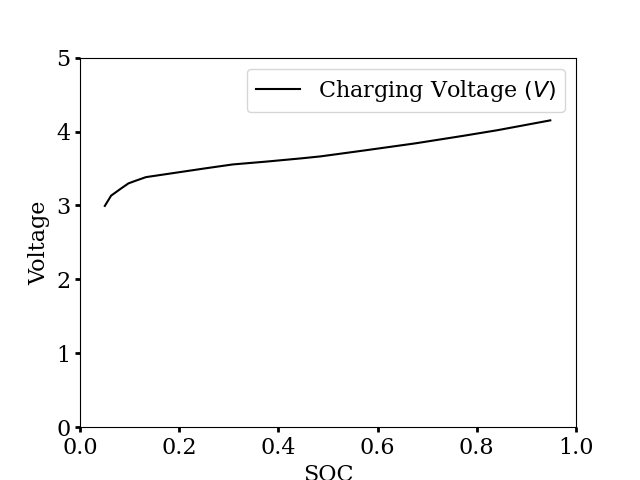
\includegraphics[scale=.4]{Chap06/Figures/PowerAnalyzerResults/Batt_Charging_Voltage_SOC.png}}\label{fig:Batt_Charging_Voltage_SOC}
	\qquad
	\subfigure[Battery Voltage Vs SOC @Discharging]{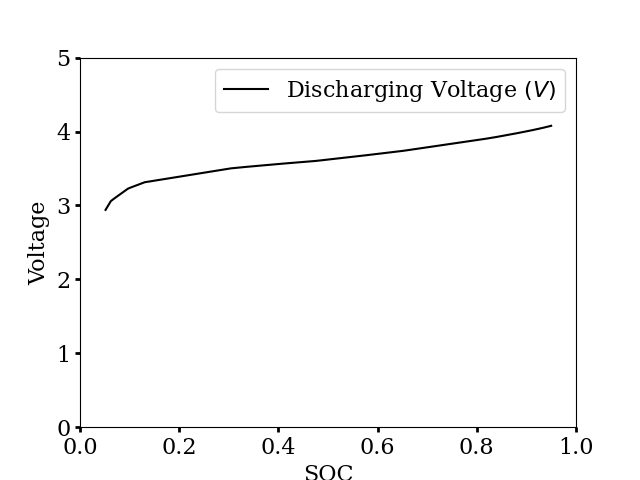
\includegraphics[scale=.4]{Chap06/Figures/PowerAnalyzerResults/Batt_Discharging_Voltage_SOC.png}}\label{fig:Batt_Discharging_Voltage_SOC}
	\qquad
	\subfigure[Battery Voltage Vs Cycles @Charging and Discharging]{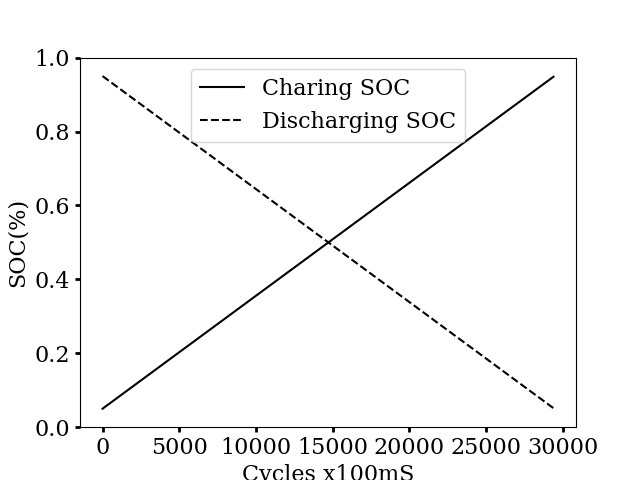
\includegraphics[scale=.4]{Chap06/Figures/PowerAnalyzerResults/Batt_Discharging_Charging_SOC_Cycles.png}}\label{fig:Batt_Discharging_Charging_SOC_Cycles}
	\qquad
	\subfigure[Battery SOC Vs Cycles @Charging and Discharging]{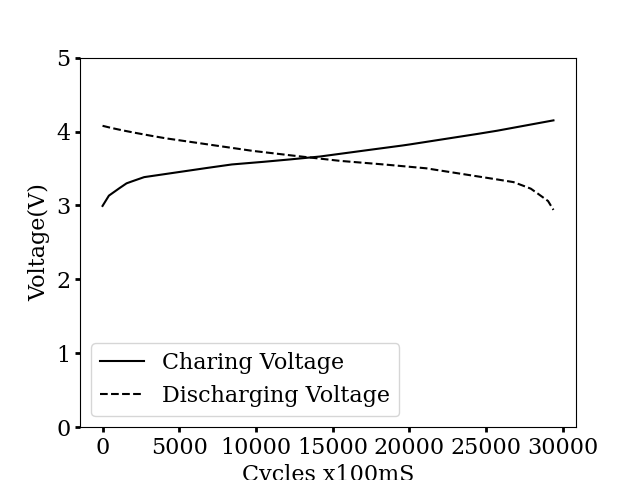
\includegraphics[scale=.4]{Chap06/Figures/PowerAnalyzerResults/Batt_Discharging_Charging_Voltage_Cycles.png}}\label{fig:Batt_Discharging_Charging_Voltage_Cycles}
	\caption{Single Battery Modeling Characteristics with PowerAnalyzer }\label{fig:Single_Batt_Modeling_Results}
\end{figure}

\begin{figure}[h]
	\centering
	\subfigure[Battery Pack Voltages Vs Cycles @Charging (same SOC)]{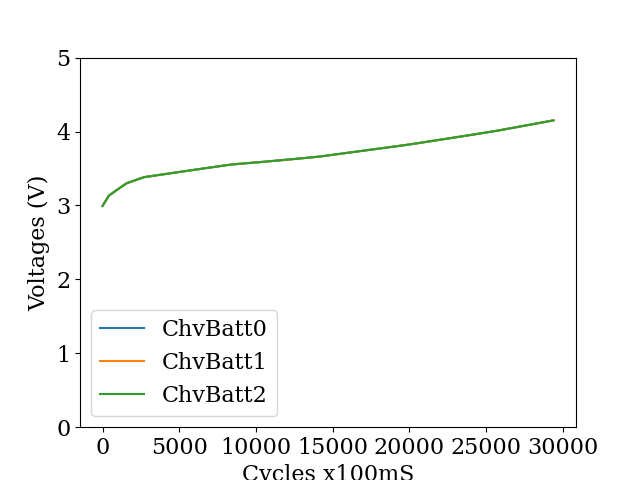
\includegraphics[scale=.4]{Chap06/Figures/PowerAnalyzerResults/Batt_Pack_Charging_Voltage_Cycles.png}}\label{fig:Batt_Pack_Charging_Voltage_Cycles}
	\qquad
	\subfigure[Battery Pack Voltages Vs Cycles @Discharging (same SOC)]{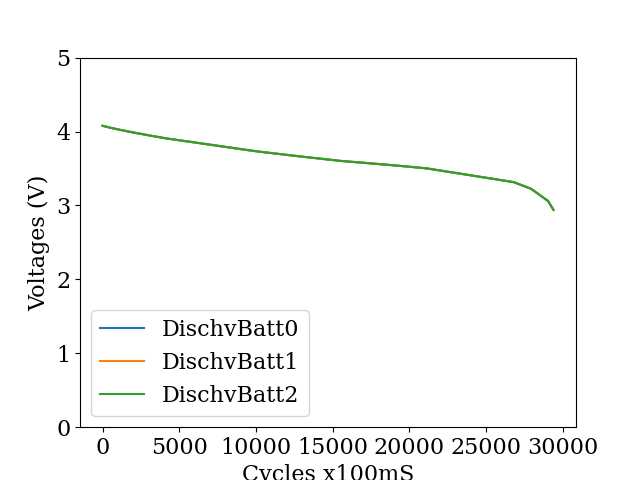
\includegraphics[scale=.4]{Chap06/Figures/PowerAnalyzerResults/Batt_Pack_Discharging_Voltage_Cycles.png}}\label{fig:Batt_Pack_Discharging_Voltage_Cycles}
	\qquad
	\subfigure[Battery Pack SOCs Vs Cycles @Charging and Discharging (same SOC)]{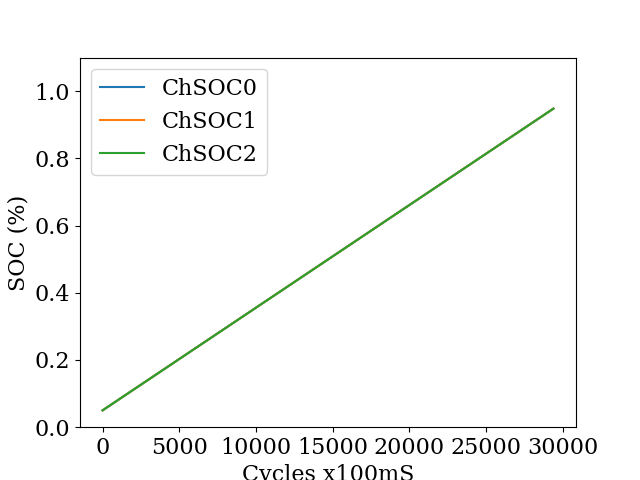
\includegraphics[scale=.4]{Chap06/Figures/PowerAnalyzerResults/Batt_Pack_Charging_SOC_Cycles.png}}\label{fig:Batt_Pack_Charging_SOC_Cycles}
	\qquad
	\subfigure[Battery Pack SOCs Vs Cycles @Charging and Discharging (same SOC)]{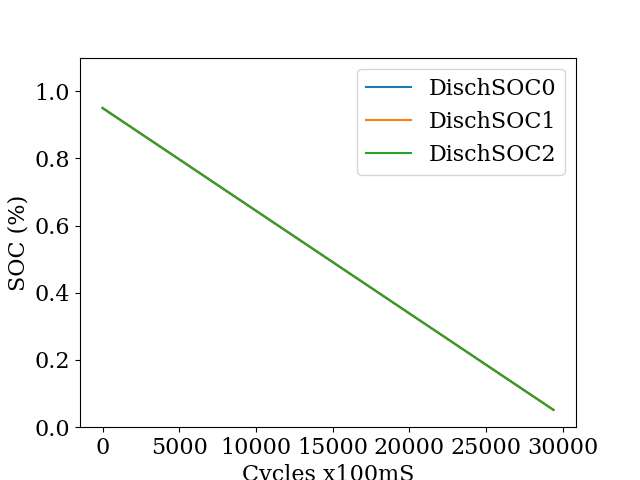
\includegraphics[scale=.4]{Chap06/Figures/PowerAnalyzerResults/Batt_Pack_Discharging_SOC_Cycles.png}}\label{fig:Batt_Pack_Discharging_SOC_Cycles}
	\qquad
	\subfigure[Battery Pack SOCs Vs Cycles @Charging(Different SOC)]{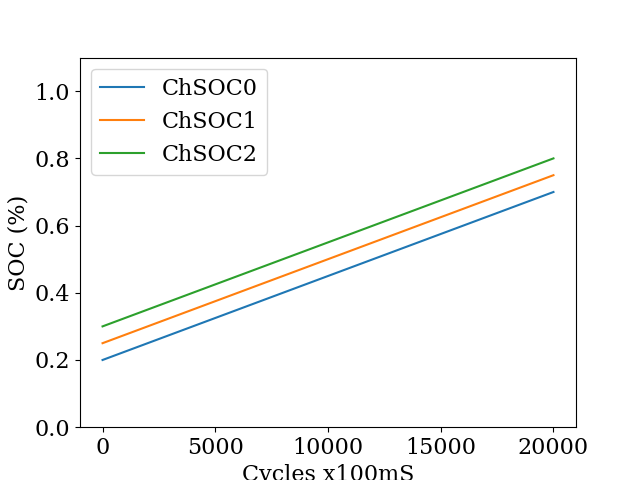
\includegraphics[scale=.4]{Chap06/Figures/PowerAnalyzerResults/Batt_Pack_Diff_SOC_Charging_SOC_Cycles.png}}\label{fig:Batt_Pack_Diff_SOC_Charging_SOC_Cycles}
	\qquad
	\subfigure[Battery Pack SOCs Vs Cycles @Charging(Different SOC)]{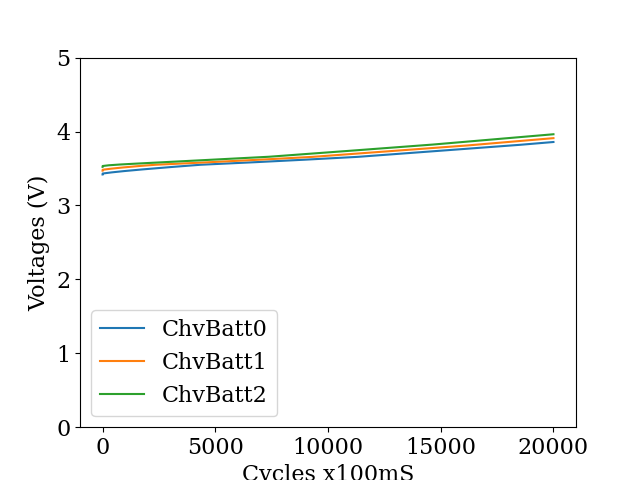
\includegraphics[scale=.4]{Chap06/Figures/PowerAnalyzerResults/Batt_Pack_Diff_SOC_Charging_Voltage_Cycles.png}}\label{fig:Batt_Pack_Diff_SOC_Charging_Voltage_Cycles}
	\caption{Battery Pack Modeling Characteristics with PowerAnalyzer(3 Cells) } \label{fig:Batt_Pack_Modeling_Results}
\end{figure}

The results in \ref{fig:Single_Batt_Modeling_Results} will enrich the battery modeling and power analyzer implementation, the data shown in the figure  \ref{fig:Single_Batt_Modeling_Results} will collect for one single battery with a one-time constant model. The data has been collected for one single battery from full charge to discharge, soc is from $5\%$ to $95\%$, and vice versa. The obtained results of battery voltage Vs SoC must match with the Voltage Soc curve provided by the manufacturer.
The charging voltage and soc \ref{fig:Single_Batt_Modeling_Results}(a) (discharging \ref{fig:Single_Batt_Modeling_Results}(b)) of the battery impressively match the results provided by the manufacturer in the voltage SoC graph \ref{fig:Battery_OCV_Vs_Soc}. 
Undoubtedly the battery modeling \ref{fig:Single_Batt_Modeling_Results} results match the OCV curve of the battery \ref{fig:Single_Batt_Modeling_Results}(a) and \ref{fig:Single_Batt_Modeling_Results}(b), yet it is very important to consider the symmetry of the OCV curve during charging and discharging Figure \ref{fig:Single_Batt_Modeling_Results}(c) and \ref{fig:Single_Batt_Modeling_Results}(d). The charging and discharging of curves of the battery are symmetry about $47\%$ of the SoC, which is a good sign for an estimate of the battery soc both at charging and discharging.
Figure \ref{fig:Single_Batt_Modeling_Results}(c) and \ref{fig:Single_Batt_Modeling_Results}(d)  plotted battery voltage and SoC vs cycles, several consecutive sampling times between the measurements are cycles. The sampling $dt$ time in this project has used multiples of 100mS. Nevertheless, $dt$ is the independent choice for the user which again depends on the application.

The target of the battery modeling is to build the battery pack with sophisticated control over it for BMS applications. Results in Figure \ref{fig:Batt_Pack_Modeling_Results} achieved such a target, I have implemented for 8 batteries (The Figures show only 3 battery results, to avoid clumsiness in the graphs).
The battery pack results are pretty much the same as results collected for a single battery Figures \ref{fig:Batt_Pack_Modeling_Results}(a) and \ref{fig:Batt_Pack_Modeling_Results}(d) show results for 8 batteries simulated with the same SOC assigned for all batteries. Thanks to the power analyzer, which will allow several battery tests for instance keep different socs and perform battery balancing, battery low and high voltage cut off. Figures \ref{fig:Batt_Pack_Modeling_Results}(e) and \ref{fig:Batt_Pack_Modeling_Results}(f) shows one such example of keeping different socs charging the batteries.

\section{Summery of Chapter \ref{ch:Battery_Modeling_Emulation}}
Part I of the chapter \ref{ch:Battery_Modeling_Emulation} described the mathematical modeling of the battery with One-time and two-time constant equivalent circuit components. An extended subsection of Part I helped to estimate the OTC and TTC model parameters with the SOC curve which became the fundamental base for the battery pack power analyzer design. Part I also briefed about the discrete-time implementation of the OTC and TTC model for the battery. The discrete-time OTC and TTC model equations are useful for estimating the battery soc with advanced algorithms like Kalman, extended Kalman, and Columb-Extended Kalman. The most satisfactory conclusion in Part I can be seen in Part II, implementing battery models with the script and emulating with lab instruments. Nonetheless, for a more analytical and mathematical understanding of batteries, I diverted read attention toward the reference papers mentioned in the Bibliography. Part II talks about the practical implementation of Part I in terms of script and different instruments. Starting subsection of Part II walks through several instruments' specifications and configurations used in this project. This chapter is indeed a bit lengthy and diversified. Because battery modeling and implementation got to go together which is the reason I took extra liberty to extend this chapter more descriptive.
I got less opportunity to describe the script but I have pushed everything to GitHub and referenced the links in miscellaneous.

To sum up the results came out from this chapter are convincing, and this can be still pursued further to develop a sophisticated graphical interface for the application. In the battery modeling, I have used the Columb counting approach for estimating the battery SOC, this can be still dragged into higher algorithms and can also increase the robustness of the model by adding more and more battery time constant models.